\section{Main Processor} \label{sec:MainProcessor}

The stored samples inside the sample control module will be retrieved by the main processor module through a parallel bus. The main processor module will perform spectral analysis on the samples and use these calculations to retrieve the magnitude and phase of the impedance. The module will then calculate all the derived quantities described in section \refq{subsec:DerivedQuantities} and transmit them to the UI module. The main processor module is shown on figure \refq{fig_6_4_MainprocessorModule}.

\begin{figure}[H]
    \centering
    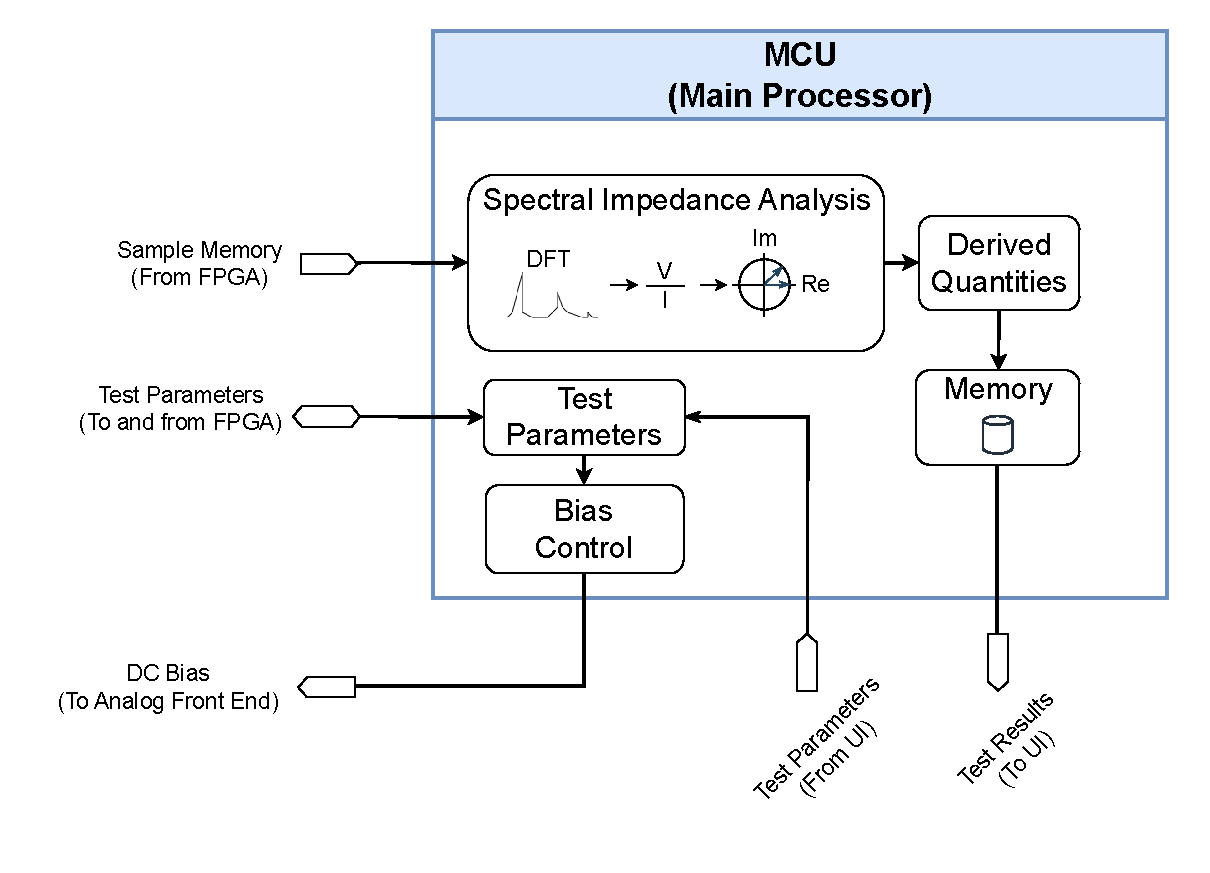
\includegraphics[clip, trim=18 0 18 0,width=0.70\textwidth]{Sections/6_SystemArchitecture/Figures/MCU.pdf}
    \caption{The main processor module takes the samples from the sample control modules memory and analyzes the samples in order to calculate the derived quantities and transmit them to the user interface module.}
    \label{fig_6_4_MainprocessorModule}
\end{figure}

The main processor module will also generate the DC bias voltage that is used inside the analog front end in order to bias the DUT. The module will, along with the DC bias, transmit all the relevant test parameters to the FPGA. The test parameters can be parameters such as test frequency, DC bias level, sample size and so on. The user can choose many of these test parameters in the UI module and the main processor module will take these choices and send them to the relevant modules.
